\textbf{\underline{OZ 3 - De Lorentzkracht en de wet van Ampère - Oefening 2:}}
\vspace{0.5cm}

% \begin{description}[labelwidth=1.5cm, leftmargin=!]
%     \item[Geg. :]   
%     \item[Gevr. :]  
%     \item[Opl. :]  
% \end{description}

Een zeer groot geleidend vlak met dikte t draagt een uniforme stroomdichtheid $\Vec{j}$. Bepaal het magneetveld (grootte, richting en zin) op een afstand $y$ boven het vlak. (Neem aan dat het vlak oneindig groot is)

% \begin{center}
%     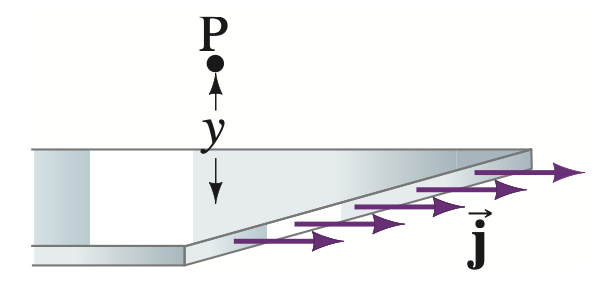
\includegraphics[scale = 0.4]{oz03/resources/Oz3Oef2.png}
% \end{center}

\begin{description}[labelwidth=1.5cm, leftmargin=!]
    \item[Geg. :] $t$, $\Vec{j}$, $y$
    \item[Gevr. :]  $\Vec{B}$ ?
    \item[Opl. :]
    \item[]
        \vspace{-0.7cm}
        \begin{minipage}{0.69\textwidth}
            The sheet may be treated as an infinite number of parallel wires. The magnetic field at a location y above the wire will be the sum of the magnetic fields produced by each of the wires. If we consider
            the magnetic field from two wires placed symmetrically on either side of where we are measuring the magnetic field, we see that the vertical magnetic field components cancel each other out. 
            Therefore, the field above the wire must be horizontal and to the left.  By symmetry, the field a location y below the wire must have the same magnitude, but point in the opposite direction. We calculate the magnetic field using Ampere’s law with a rectangular loop that extends a distance y above and below the current sheet, as shown in the figure.
            \begin{align*}
                \oint \Vec{B} \cdot d\Vec{\ell} = 2B_{\parallel}D &= \mu_0 I_{\text{in}} = \mu_0 (jtD) \\
                B_{\parallel} &= \tfrac{1}{2}\mu_0jt
            \end{align*}
        \end{minipage}
        \begin{minipage}{0.27\textwidth}
            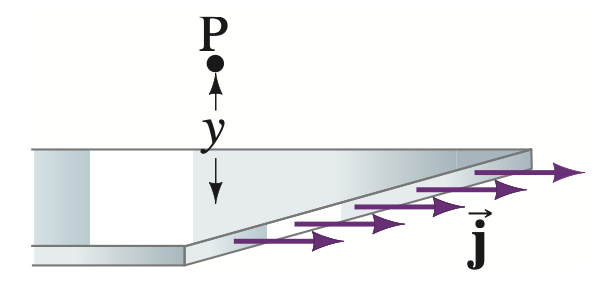
\includegraphics[scale = 0.4]{oz03/resources/Oz3Oef2.png} 
            \vspace{1cm}
            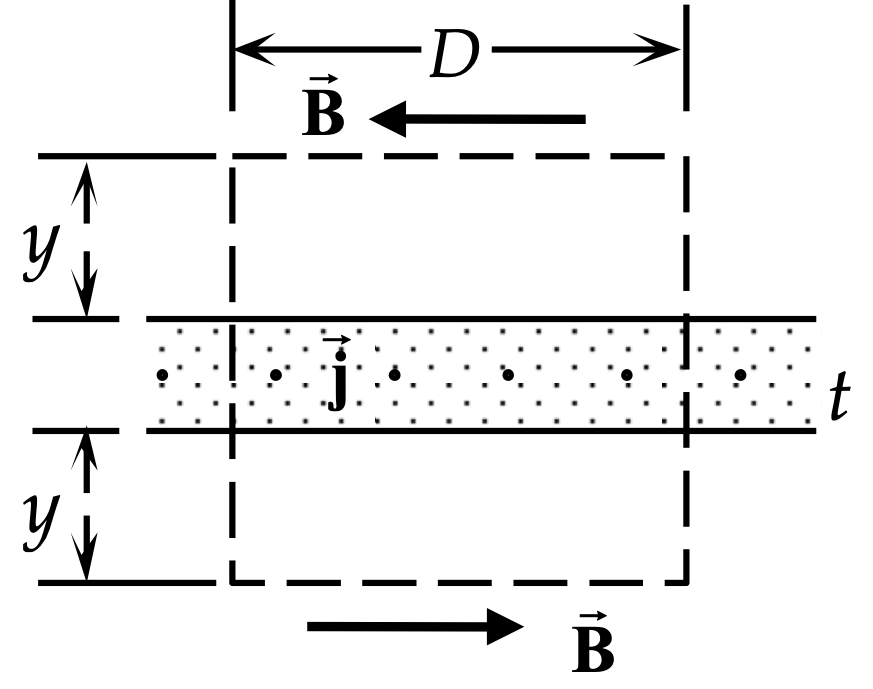
\includegraphics[scale = 0.275]{oz03/resources/Oz3Oef2Tekening.png}
        \end{minipage}

\end{description}

\vspace{1cm}